\documentclass[11pt]{article}
\usepackage{geometry}                % See geometry.pdf to learn the layout options. There are lots.
\geometry{letterpaper}                   % ... or a4paper or a5paper or ... 
%\geometry{landscape}                % Activate for for rotated page geometry
%\usepackage[parfill]{parskip}    % Activate to begin paragraphs with an empty line rather than an indent
\usepackage{graphicx}
\usepackage{amssymb}
\usepackage{amsmath}
\usepackage{epstopdf}
\usepackage{hyperref}
\DeclareGraphicsRule{.tif}{png}{.png}{`convert #1 `dirname #1`/`basename #1 .tif`.png}


\graphicspath{
{/Users/Andy/Cruises_Research/Analysis/Andy_Pickering/eq14_patch_gamma/figures/}
}

\title{Patch/Gamma Analysis for EQ14 chameleon patches}
\author{Andy Pickering}
%\date{}                                           % Activate to display a given date or no date



\begin{document}
\maketitle

\tableofcontents
\newpage

%~~~~~~~~~~~~~~~~~~~~~
\section{Overview}

The goal of this analysis is to compute mixing `coefficident' $\gamma_{\chi\epsilon}=\frac{N^2 \chi}{2\epsilon T_{z}^{2}} $ for patches in EQ14 chameleon profiles, and see if we obtain values close to $\gamma_{\chi\epsilon}=0.2$.

%~~~~~~~~~~~~~~~~~~~~~
\section{Data}

Data are made by the `Chameleon' microstructure profiler near the equator during the `EQ14' experiment. The data was shared with me by Sally/Jim. My copy is located at : 
\newline
\verb+/Users/Andy/Cruises_Research/ChiPod/Cham_Eq14_Compare/+
\medskip

Chameleon data already processed by Sally is in : \newline
\verb+/Users/Andy/Cruises_Research/ChiPod/Cham_Eq14_Compare/Data/chameleon/processed/+

\medskip

This analysis is in the main folder: \newline  \verb+/Users/Andy/Cruises_Research/Analysis/Andy_Pickering/eq14_patch_gamma/+ . This is also a github repository.






%~~~~~~~~~~~~~~~~~~~~~~~~~~~~~~~~~~~~~~
\section{Methods}

\begin{itemize}

\item \verb+FindPatches_eq14_Raw.m+ Identifies patches in the profiles made by \verb+Process_tiwe_rawprofiles_AP.m+, using potential temperature.

\item \verb+Compute_N2_dTdz_patches_eq14_eachcast.m+ Computes $N^2$ and $T_z$ for patches, using several different methods. SAves results in a structure `patches'.

\item \verb+add_binned_to_patches.m+

\item \verb+run_eq14_for_PATCHES.m+ Runs the Chameleon processing (including $\chi$ and $\epsilon$) for just the patches identified in \verb+FindPatches_eq14_Raw.m+ . This calls \verb+average_data_PATCH_AP.m+ instead of \verb+average_data_gen1.m+.

\item \verb+add_patch_chi_eps_to_patches_eq14_each_profile.m+ Adds  $\chi$ and $\epsilon$ comptued over patches (in \verb+run_eq14_for_PATCHES.m+ ) to patch profiles.

\item \verb+combine_patch_profiles_eq14.m+ Combines all patch profiles into 1 structure.


\end{itemize}

\medskip

%~~~~~~~
\subsection{dTdz}

Temperature gradient is computed for each patch using the following methods:
\begin{enumerate}
\item $dtdz_{range}$ : Take the range of T over the patch and divided by patch height
\item $dtdz_{line}$ : Fit a straight line to sorted T using \verb+polyfit+
\item $dtdz_{bulk}$ : Use the 'bulk gradient' from Smyth et al 2001, which is the rms fluctuation from the background (sorted) temperature, divided by the thorpe scale (the rms re-ordering distances).
\end{enumerate}


%~~~~~~~
\subsection{N2}

$N^2$ is computed for each patch using the following methods:
\begin{enumerate}
\item $N^2_{range}$ : Take the range of potential density over the patch divided by the patch height ($d\rho/dz$), then compute $N^2=\frac{-g}{\rho_o}\frac{d\rho}{dz}$ where $\rho_o$ is the mean potential density over the patch.
\item $N^2_{line}$ : Fit a straight line to sorted potential density using polyfit to get $d\rho/dz$, then compute N2.
\item $N^2_{bulk}$ : Use 'bulk gradient' . This is calculated from the bulk $T_z$, using a linear fit between density and temperature.
\item $N^2_4$ : Compute $N^2$ from the sorted profile (sorted by potential density) using \verb+sw_bfreq+, then take average over the patch. I believe this method is used by some commonly-used overturn codes.
\end{enumerate}


%~~~~~~~
\subsection{Mixing Efficiency}

Mixing Efficiency $\gamma_{\chi\epsilon}$ is computed from the following equation using differerent $N^2$ and $dT/dz$ values.
\begin{equation}
\gamma_{\chi\epsilon}=\frac{N^2 \chi}{2\epsilon T_{z}^{2}} 
\end{equation}
$\chi$ and $\epsilon$ are computed over each patch from the Chameleon data. Gamma is computed for the following 4 combinations:
\begin{enumerate}
\item  $\gamma_{range}$ : N^{2}_{range}$, $dtdz_{range}$
\item  $\gamma_{line}$ : N^{2}_{line}$, $dtdz_{line}$
\item  $\gamma_{bulk}$ : N^{2}_{bulk}$, $dtdz_{bulk}$
\item  $\gamma_{range}$ : N^{2}_{4}$, $dtdz_{line}$
\end{enumerate}
Values where $\epsilon$ is below the noise floor of $log_{10}[\epsilon]=-8.5$ are discarded.





%~~~~~~~~~~~~~~~~~~~~~~~~~~~~~~~~~~~
\section{Results}

\begin{itemize}
\item $\gamma_{\chi\epsilon}$ computed for 1m avg data is about an order of magnitude less than $0.2$ (Figure \ref{avggam}). The data was processed by Sally w/ 2 different c-star values, this doesn't seem to make any difference in the estimated $\gamma_{\chi\epsilon}$.
\item $\gamma_{\chi\epsilon}$ computed for just patches is about an order of magnitude less than $0.2$ (Figure \ref{patchgam}).
\end{itemize}


% gamma for all binned data
\begin{figure}[htbp]
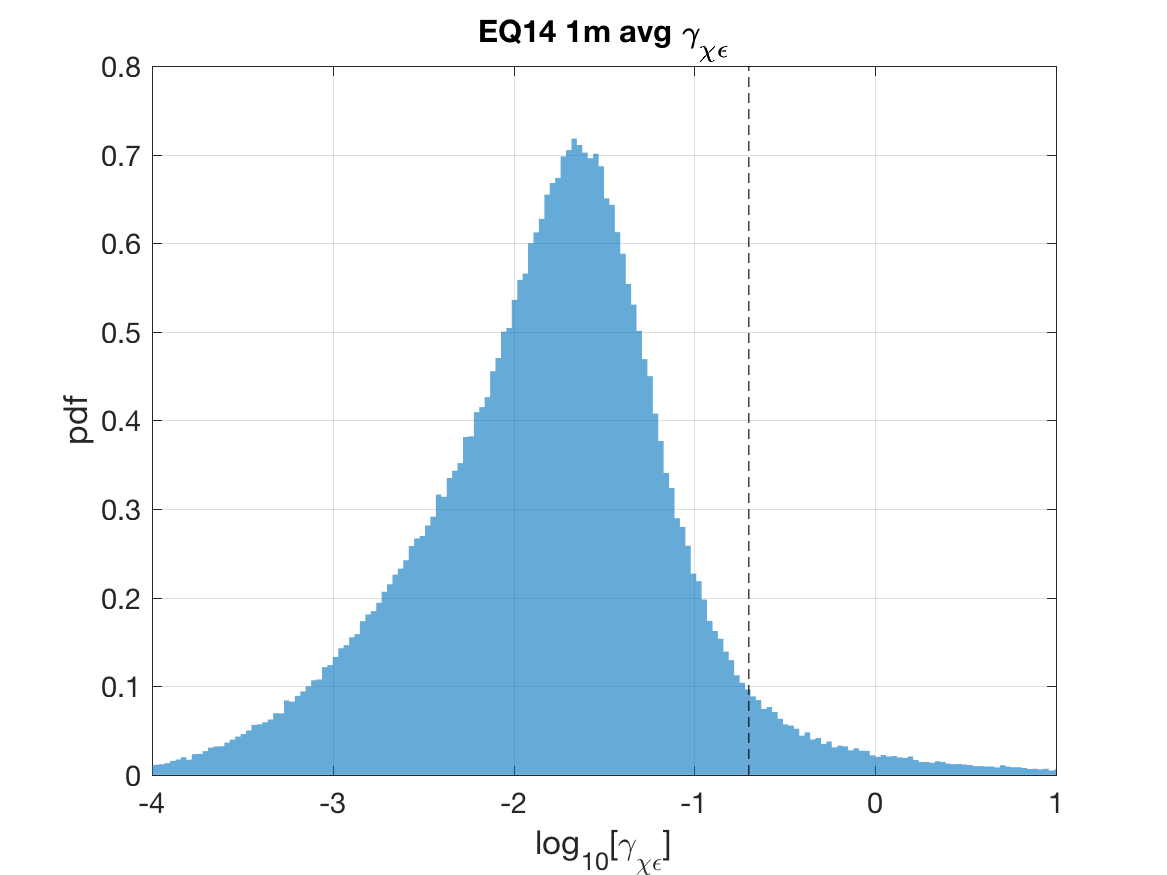
\includegraphics[scale=0.8]{eq14_binned_gamma.png}
\caption{Histogram of $\gamma_{\chi\epsilon}$ for 1m avg chameleon profiles. Vertical dashed line shows $\gamma=0.2$.}
\label{avggam}
\end{figure}

% gamma for just patches
\begin{figure}[htbp]
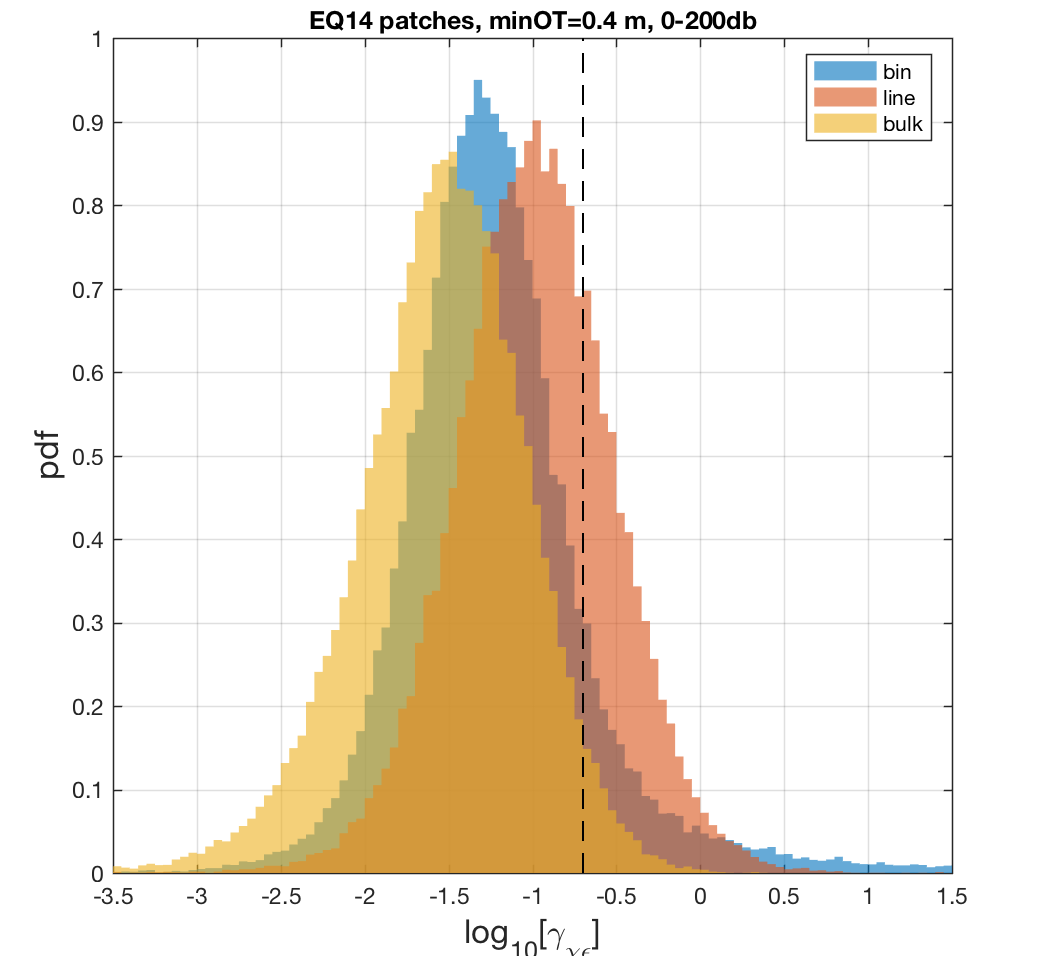
\includegraphics[scale=0.8]{eq14_minOT_40_usetemp_1_gammas_hist_cast_1_3100_zrange_0_200.png}
\caption{Histogram of $\gamma_{\chi\epsilon}$ for patches, using different estimates of $N^2$ and $T_z$. Vertical dashed line shows $\gamma=0.2$. For all profiles, all depths.}
\label{patchgam}
\end{figure}

\begin{figure}[htbp]
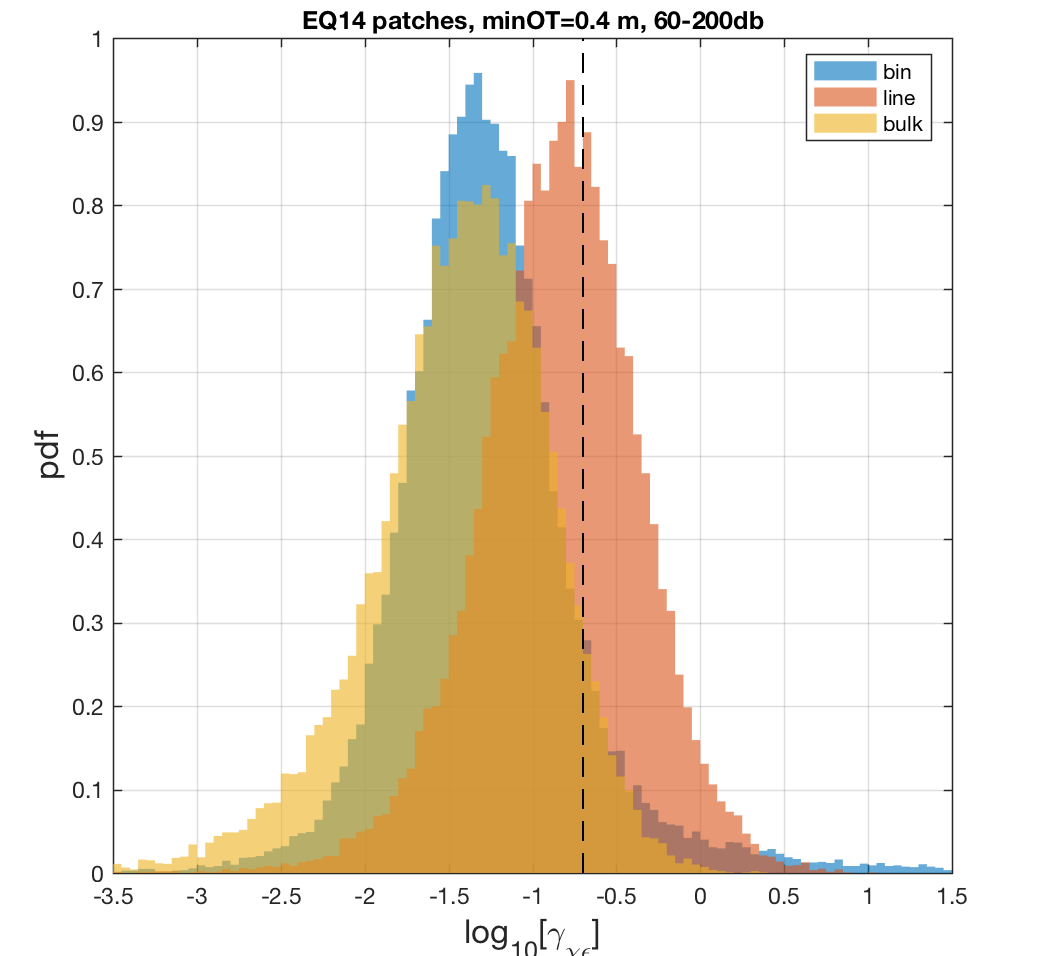
\includegraphics[scale=0.8]{eq14_minOT_40_usetemp_1_gammas_hist_cast_1_3100_zrange_60_200.png}
\caption{Histogram of $\gamma_{\chi\epsilon}$ for patches, using different estimates of $N^2$ and $T_z$. Vertical dashed line shows $\gamma=0.2$. For all profiles, depths 60-200m only.}
\label{patchgam}
\end{figure}


%~~~~~~~~~~~
\subsection{Using smaller fmax?}

I believe the Chameleon data processed by Sally used the standard fmax=32Hz correction/cutoff for the thermistor data. However when I was trying to apply the $\chi$pod method to that data, I looked at some spectra and it looked like the thermistor rolled off much lower, around maybe 7-10hz. So I re-ran the processing using fmax=7hz. Estimates of $\gamma_{\chi\epsilon}$ are about 2-3 times larger (Figure \ref{avggam7hz}), but still significantly less than 0.2 .

% plot of binned gamma using fmax=7?
% gamma for all binned data
\begin{figure}[htbp]
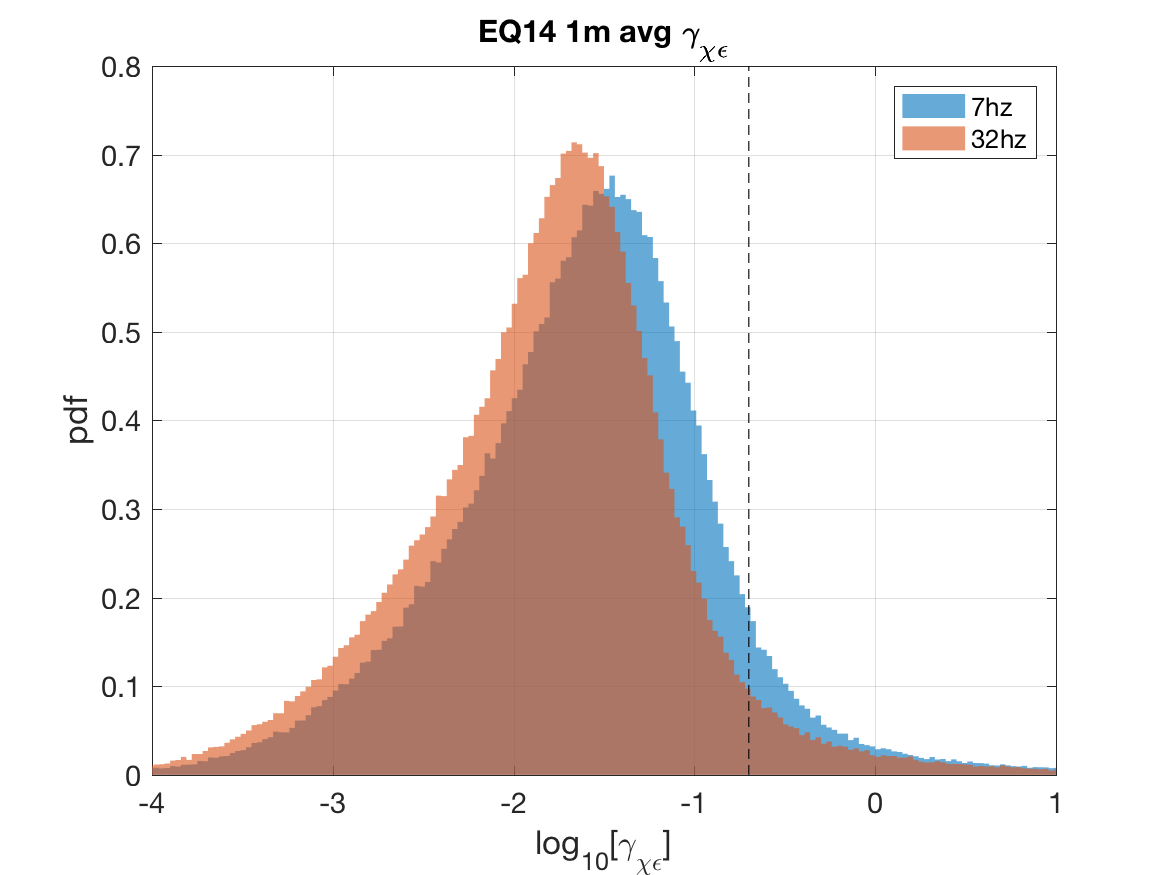
\includegraphics[scale=0.8]{eq14_binned_gamma_7hz.png}
\caption{Histogram of $\gamma_{\chi\epsilon}$ for 1m avg chameleon profiles, for standard fmax32hz as well as fmax7hz. Vertical dashed line shows $\gamma=0.2$.}
\label{avggam7hz}
\end{figure}




\clearpage
%~~~~~~~~~~~~~~~~
\subsection{Variation of $\gamma_{\chi\epsilon}$ over time}

To investigate whether $\gamma_{\chi\epsilon}$ varies over time, I plotted $\gamma_{\chi\epsilon}$ vs cast number (Figure \ref{gamvscnum}).

\begin{figure}[htbp]
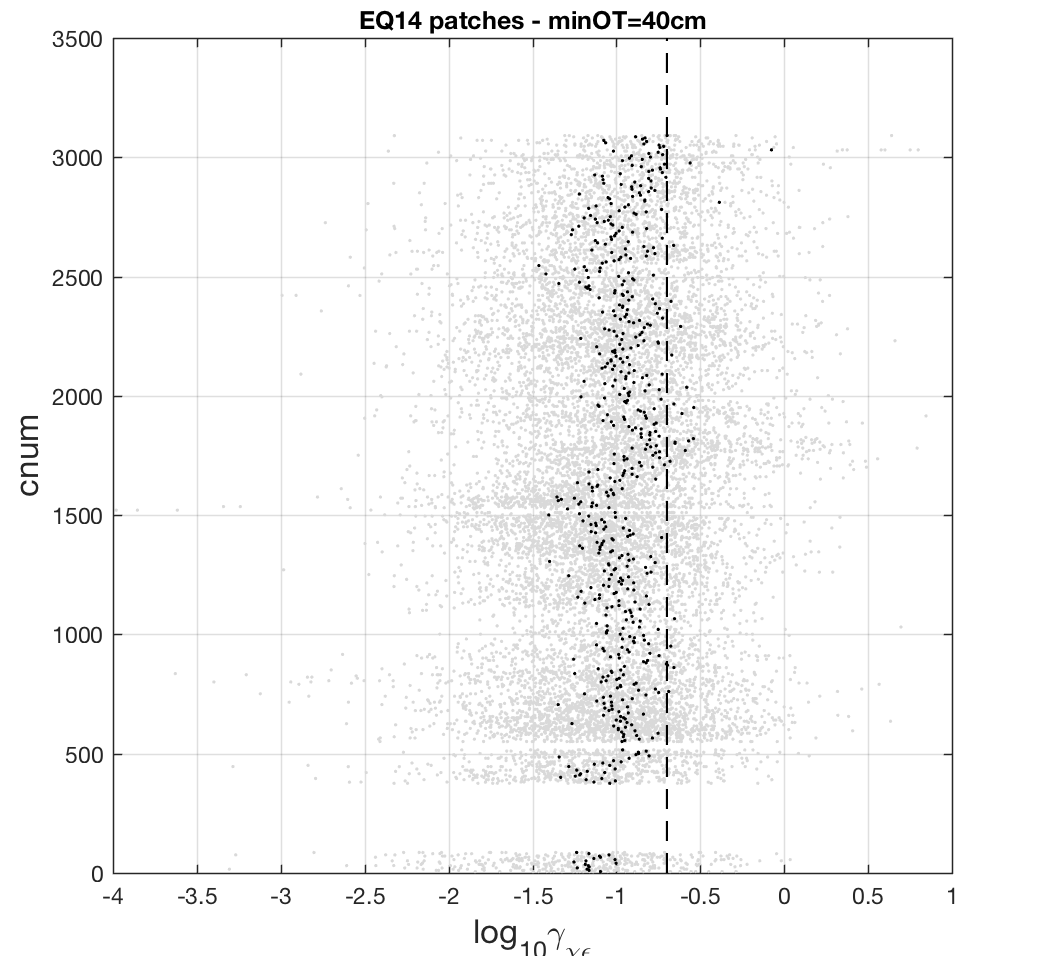
\includegraphics[scale=0.8]{eq14_minOT_40_usetemp_1_gam_vs_cnum.png}
\caption{Plot of $\gamma_{\chi\epsilon}$ for patches vs cast number. Vertical line is $\gamma=0.2$. Black points are the median value for each cast.}
\label{gamvscnum}
\end{figure}



\clearpage
%~~~~~~~~~~~~~~~~
\subsection{Variation of $\gamma_{\chi\epsilon}$ over depth?}

\verb+plot_gamma_vs_depth_eq14.m+


\begin{figure}[htbp]
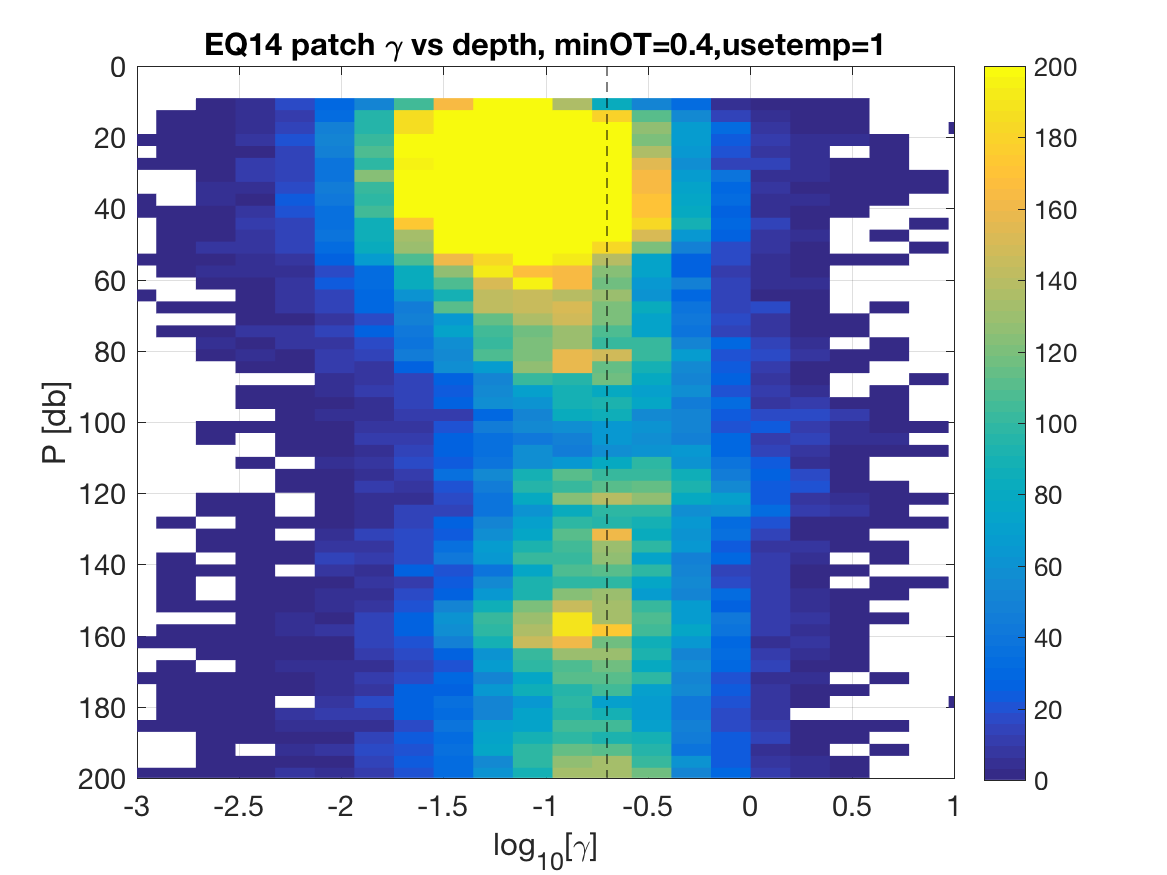
\includegraphics[scale=0.8]{eq14_patch_gamma_minOT_40_usetemp_1_gammas_vs_depth.png}
\caption{Plot of $\gamma_{\chi\epsilon}$ for patches? vs depth. Vertical line is $\gamma=0.2$. }
\label{gamvsdepth}
\end{figure}







\clearpage
%~~~~~~~~~~~~~~~~~~~~~~~~~~~~~~~~~~~~~~~~
\section{Summary}

\begin{itemize}
\item $\gamma_{\chi\epsilon}$ computed from 1m binned data (the standard Chameleon processing) is about 10 times smaller than the typical assumed value of 0.2.
\item $\gamma_{\chi\epsilon}$ computed for just patches is larger. If only depth range 60-200m used, gamma using `line' method is about 0.2.
\item $\gamma_{\chi\epsilon}$ does not appear to vary much over time/cast number, as was seen in tiwe data.
\end{itemize}



\end{document}  


